\section{Auswertung}
\label{sec:Auswertung}
\subsection{Entladevorgang eines Kondensators}
Bei der ersten Methode zur Bestimmung der Zeitkonstante wird der Entladevorgang eines Kondensators über einen Widerstand in der Abbildung \ref{fig:map001} beobachtet. Die gemessenen Daten befinden sich in der Tabelle \ref{tab:EntladungKondensator}. Es werden aus der Tabelle \ref{tab:EntladungKondensator} die $31$ Wertepaare entnommen und die Spannung $U_\text{C}$ logarithmiert. 
Mit den Wertepaare  wird eine lineare Ausgleichsgerade zur Bestimmung der Zeitkonstante durchgeführt und in die Abbildung \ref{fig:zeit} eingetragen. 
\begin{figure}[h!]
	\centering
	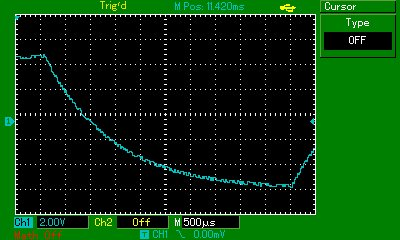
\includegraphics[width=0.7\linewidth]{../../MAP001}
	\caption{Entladevorgang eines Kondensators}
	\label{fig:map001}
\end{figure}

Eine lineare Ausgleichsgerade lässt sich berechnen wie:
\begin{equation}
\label{eqn:Regression}
y = mx+b
\end{equation}
wobei $m$ die Steigung und $b$ der y-Achsenabschnitt sind. Über Formel \ref{eqn:Meth1} lässt sich RC bestimmen. Die Steigung der Ausgleichsgeraden der Form in der Gleichung \ref{eqn:Regression} wird vom Python-Modul Matplotlib berechnet und beträgt:
\begin{align*}
m &= -\frac{1}{RC} \\
  &= \SI{-983.89 \pm 27.88}{\frac{1}{s}}
\end{align*}
mit $R$ als Widerstand und $C$ als Kapazität des Kondensators.
Der y-Achsenabschnitt ist gegeben als:
\begin{equation*}
b = ln(Q(0)) 
\end{equation*}
wobei $Q(0)$ die Ladung des Kondensators zum Zeitpunkt $t=0$ beschreibt und beträgt somit:
\begin{equation*}
b = (1.016 \pm 0.035) \text{ln(C)}.
\end{equation*}
Die Steigung lässt sich nach $RC$ umstellen und mit Hilfe des bekannten Wertes ergibt sich:
\begin{align*}
RC &= -\frac{1}{m} \\
   &= \SI{1.016 \pm 0.035}{\ms} .
\end{align*}
\begin{figure}[h!]
	\centering
	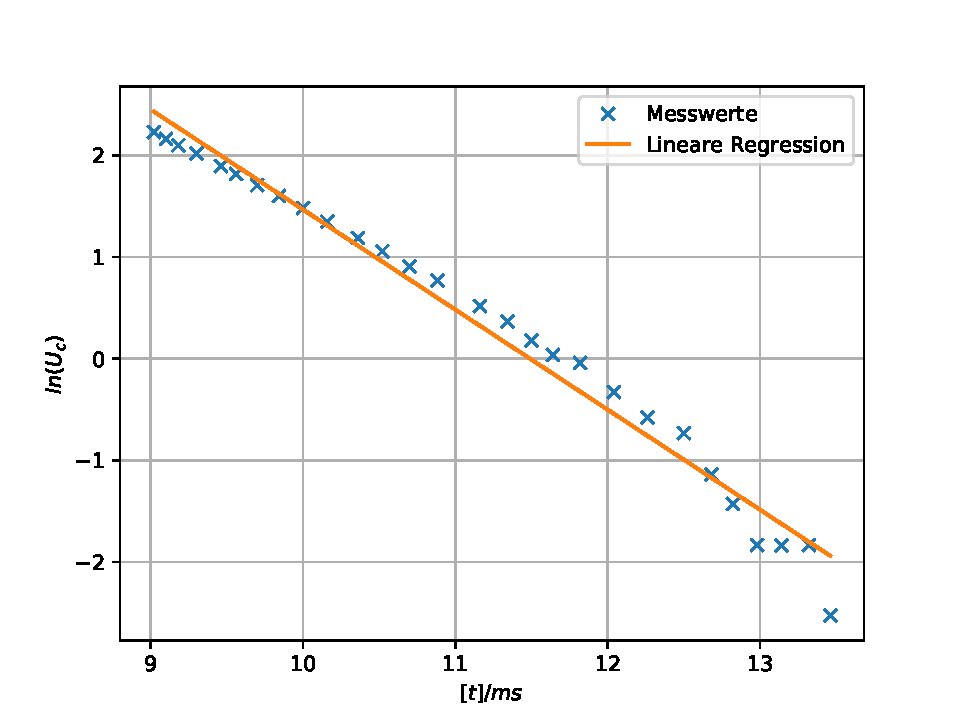
\includegraphics[width=0.9\linewidth]{../../Zeit}
	\caption{Lineare Ausgleichsgerade zur Bestimmung der Zeitkonstante}
	\label{fig:zeit}
\end{figure}
\begin{table}[htbp]
	\centering
	\caption{Messdaten zur Entladung eines Kondensators}
	\label{tab:EntladungKondensator}
	\begin{tabular}{c c}
		\toprule
		$t / \si{ms} $ & $ U_\text{C} / \si{V}$ \\
		\midrule
		9,02	& 4,08 \\
		9,10	& 3,52 \\
		9,18	& 2,96 \\
		9,30	& 2,32 \\
		9,46	& 1,44 \\
		9,56	& 0,96 \\
		9,70	& 0,32 \\
		9,84	& -0,24 \\
		10,00 & -0,80 \\
		10,16 &-1,36 \\
		10,36 &-1,92 \\
		10,52 &-2,32 \\
		10,70 &-2,72 \\
		10,88 &-3,04 \\
		11,16 &-3,52 \\
		11,34 &-3,76 \\
		11,50 &-4,00 \\
		11,64 &-4,16 \\
		11,82 &-4,24 \\
		12,04 &-4,48 \\
		12,26 &-4,64 \\
		12,50 &-4,72 \\
		12,68 &-4,88 \\
		12,82 &-4,96 \\
		12,98 &-5,04 \\
		13,14 &-5,04 \\
		13,32 &-5,04 \\
		13,46 &-5,12 \\
		13,66 &-5,20 \\
		13,92 &-5,20 \\
		\bottomrule
	\end{tabular}
\end{table}
\FloatBarrier
\subsection{Frequenzabhängigkeit der Amplitude}
Bei der zweiten Methode soll die Zeitkonstante $RC$ mit der Frequenzabhängigkeit der Amplitude $A$ am Kondensator bestimmt werden. Die Messdaten befinden sich in der Tabelle \ref{tab:Frequenzamplitude}. Mit Hilfe von den Messwerten wird eine Ausgleichsrechnung mit der Formel \ref{eq:Meth2} durchgeführt, die in der Abbildung \ref{fig:freq} zu sehen ist. Zur Vereinfachung wird die Formel \ref{eq:Meth2} umgeschrieben und es gilt:
\begin{equation}
\label{eqn:Freq}
\frac{A(\nu)}{U_0} = \frac{1}{\sqrt{1+(2 \pi \nu RC)^{2}}}
\end{equation}
wobei $U_{0}$ die Amplitude der Schwingung ist. 
Hier wird ebenfalls die Zeitkonstante vom Python-Modul Matplotlib aus der Gleichung \ref{eqn:Freq} berechnet und beträgt somit:
\begin{equation*}
RC = \SI{1.329 \pm 0.013}{\ms}.
\end{equation*}
\begin{figure}[h!]
	\centering
	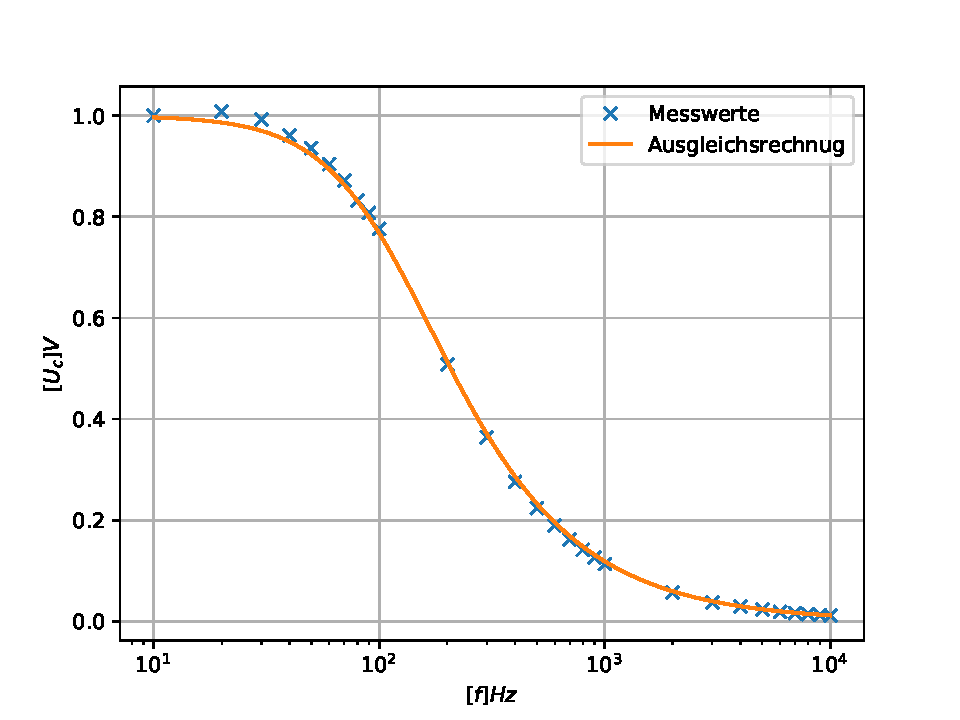
\includegraphics[width=0.9\linewidth]{../../Freq}
	\caption{Bestimmung der Zeitkonstante mit der Amplitude $A$ in Abhängigkeit der Frequenz $\nu$}
	\label{fig:freq}
\end{figure}
\begin{table}[htbp]
	\centering
	\caption{Messdaten für die Frequenzabhängigkeit der Amplitude}
	\label{tab:Frequenzamplitude}
	\begin{tabular}{c c}
		\toprule
		$\nu / \si{Hz} $ & $ U / \si{V}$ \\
		\midrule
		10	& 5,00 \\
		20	& 5,04 \\
		30	& 4,96 \\
		40	& 4,80 \\
		50	& 4,68 \\
		60	& 4,52 \\
		70	& 4,36 \\ 
		80	& 4,16 \\
		90	& 4,04 \\
		100	& 3,88 \\
		200	& 2,54 \\
		300	& 1,82 \\
		400	& 1,38 \\
		500	& 1,12 \\
		600	& 0,95 \\
		700	& 0,81 \\
		800	& 0,71 \\
		900	& 0,63 \\
		1000 &	0,568 \\
		2000 &	0,288 \\
		3000 &	0,190 \\
		4000 &	0,145 \\
		5000 &	0,116 \\
		6000 &	0,082 \\
		7000 &	0,082 \\
		8000 &	0,072 \\
		9000 &	0,064 \\
		10000 &	0,058 \\
		\bottomrule
	\end{tabular}
\end{table}
\FloatBarrier
\subsection{Frequenzabhängigkeit der Phasenverschiebung}
Bei der dritten Methode wird die $RC$-Konstante mit Hilfe der Phasenverschiebung zwischen Generator- und Kondensatorspannung bestimmt. Die Phasenverschiebung errechnet sich wie folgt:
\begin{equation}
\phi = \frac{a}{b} \cdot 2\pi
\end{equation}
wobei $a$ der zeitliche Abstand der Nulldurchgänge der Schwingungen und $b$ die Periodendauer einer Schwingung sind.
In der Tabelle \ref{tab:Frequenzphase} befinden sich die gemessenen Daten. Für die Ausgleichsrechnung wird die Formel \ref{eq:phasenverschiebung} benötigt.
Analog zu den ersten beiden Methoden werden die Wertepaare aus der Tabelle \ref{tab:Frequenzphase} entnommen und gemäß Gleichung \ref{eqn:Phase} eine Regression durchgeführt, die in der Abbildung \ref{fig:freq2} zu sehen ist.

Die Zeitkonstante $RC$ beträgt also:
\begin{equation*}
RC = \SI{1.849 \pm 0.018}{\ms}.
\end{equation*}
\begin{figure}[h!]
	\centering
	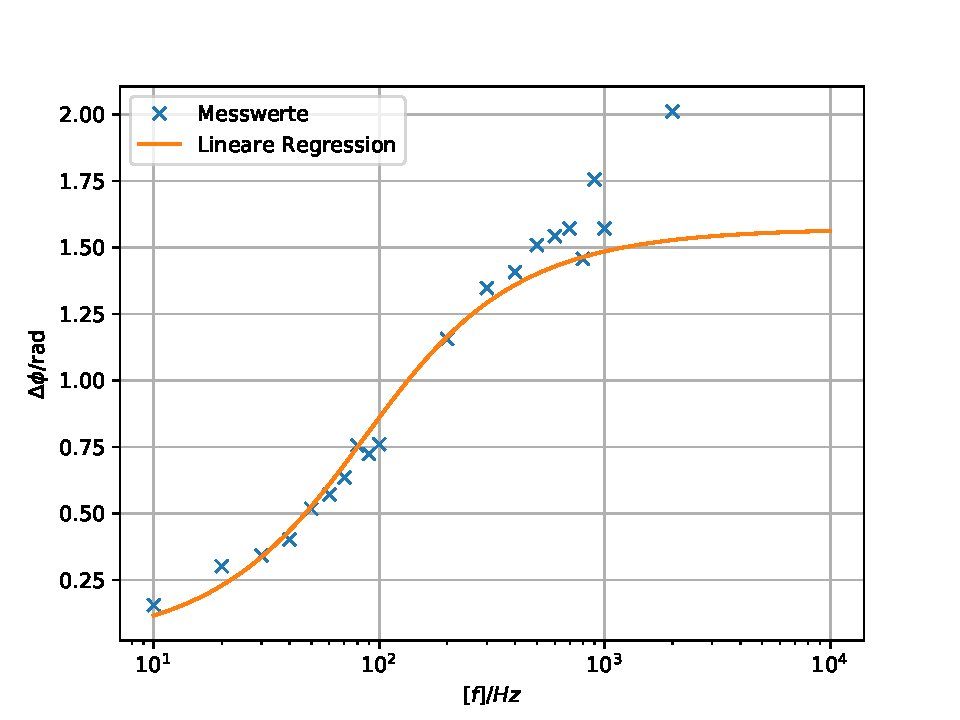
\includegraphics[width=0.9\linewidth]{../../Freq2}
	\caption{Bestimmung der Zeitkonstante unter Frequenzabhängigkeit der Phasenverschiebung}
	\label{fig:freq2}
\end{figure}
\begin{table}[htbp]
	\centering
	\caption{Messdaten für die Frequenzabhängigkeit der Phasenverschiebung}
	\label{tab:Frequenzphase}
	\begin{tabular}{c c c c}
		\toprule
		$\nu / \si{Hz} $ & $ a / \si{ms}$ & $ b / \si{ms}$ & $\phi / \text{rad}$ \\
		\midrule
	    10 & 2,40 & 97,60 & 0,154 \\
	    20 & 2,40 & 50,00 & 0,301 \\
	    30	& 1,80 & 33,20 & 0,340 \\
	    40	& 1,60& 25,00 & 0,402 \\
	    50	& 1,52 & 18,48 & 0,517 \\
	    60	& 1,52 & 16,72 & 0,577 \\
	    70	& 1,44 & 14,24 & 0,635 \\
	    80	& 1,52 & 12,64 & 0,755 \\
	    90	& 1,28 & 11,12 & 0,723 \\
	    100	& 1,20 & 9,92 & 0,760 \\
	    200	& 0,92 & 5,00 & 1,156 \\
	    300	& 0,72 & 3,36 & 1,346 \\
	    400	& 0,56 & 2,50 & 1,407 \\
	    500	& 0,48 & 2,00 & 1,507 \\
	    600	& 0,41 & 1,67 & 1,542 \\
	    700	& 0,36 & 1,44 & 1,570 \\
	    800	& 0,29 & 1,25 & 1,457 \\
	    900	& 0,31 & 1,11 & 1,754 \\
	    1000 & 0,25 & 1,00 & 1,570 \\
	    2000 & 0,16 & 0,50 & 2,010 \\
		\bottomrule
	\end{tabular}
\end{table}
\FloatBarrier
\subsection{Beobachtung der Phasenverschiebung zwischen der Generator- und Kondensatorspannung}
Mit Hilfe der Daten aus der Tabelle  lässt sich ein Polarplot erstellen, der in Abbildung \ref{fig:polar} zu sehen ist. 
\begin{figure}[h!]
	\centering
	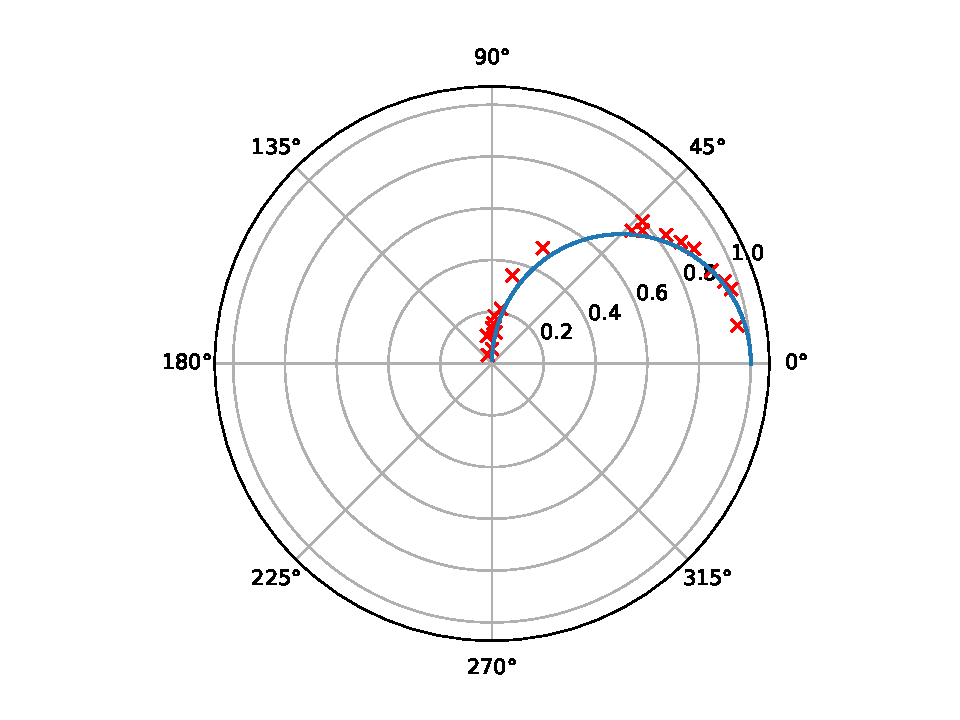
\includegraphics{../../Polar}
	\caption{Polarplot zur Beobachtung der Phasenverschiebung zwischen der Generator- und Kondensatorspannung }
	\label{fig:polar}
\end{figure}
\begin{table}[htbp]
	\centering
	\caption{Messdaten zur Beobachtung der Phasenverschiebung zwischen der Generator- und Kondensatorspannung}
	\label{tab:Polarplot}
	\begin{tabular}{c c}
		\toprule
		$\frac{A}{U_0} $ & $\phi / \text{rad}$ \\
		\midrule
		0,959 &	0,154 \\
		0,967 &	0,301 \\
		0,952 &	0,340 \\
		0,921 &	0,402 \\ 
		0,898 &	0,516 \\
		0,867 &	0,571 \\
		0,836 &	0,635 \\
		0,798 &	0,755 \\
		0,775 &	0,723 \\
		0,744 &	0,760 \\
		0,487 &	1,156 \\
		0,349 &	1,346 \\
		0,214 &	1,407 \\
		0,182 &	1,507 \\
		0,155 &	1,542 \\
		0,136 &	1,570 \\
		0,120 &	1,457 \\
		0,109 &	1,754 \\
		0,055 &	1,570 \\
		0,036 &	2,010 \\
		\bottomrule
	\end{tabular}
\end{table}
\FloatBarrier
\subsection{RC-Kreis als Integrator}
Der RC-Kreis kann unter bestimmten Voraussetzungen als Integrator arbeiten. Es lässt sich eine hohe Frequenz einstellen, die in diesem Versuch $\SI{3000}{\Hz}$ beträgt. Die gelbe Funktion ist die Ausgangsspannung und die blaue Funktion ist die Spannung über den RC-Kreis. 
In der Abbildung \ref{fig:map002} wurde aus der Sinusspannung eine Cosinusspannung, zunächst aus der Rechteckspannung in der Abbildung \ref{fig:map004} eine konstant steigende Funktion und aus der Dreieckspannung in \ref{fig:map003} eine Parabel. 
Es wird also bei allen ausgegeben Bildern gezeigt, dass der RC-Kreis auch als Integrator funktionieren kann.
\begin{figure}[h!]
	\centering
	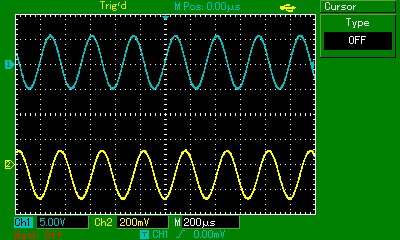
\includegraphics[width=0.6\linewidth]{../../MAP002}
	\caption{RC-Kreis, Sinusschwingung}
	\label{fig:map002}
\end{figure}
\begin{figure}[h!]
	\centering
	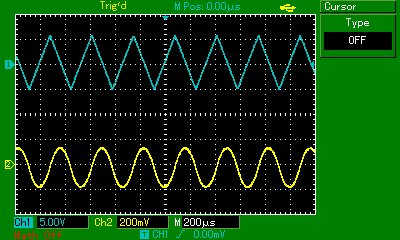
\includegraphics[width=0.6\linewidth]{../../MAP003}
	\caption{RC-Kreis, Dreieckschwingung}
	\label{fig:map003}
\end{figure}
\begin{figure}[h!]
	\centering
	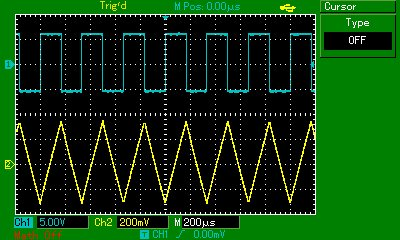
\includegraphics[width=0.6\linewidth]{../../MAP004}
	\caption{RC-Kreis, Rechteckschwingung}
	\label{fig:map004}
\end{figure}
